\chapter{Uncertainty in atomic force predictions}
\label{chapter3}

The reliability of machine-learned interatomic potentials depends not only on the accuracy of reproducing reference quantum mechanical data but also on the ability of such models to quantify uncertainty in predictions, as the desired applications of such ML models are for (large) systems that ground-truth data is inaccessible due to prohibitive scaling and the limits of computational efficiency.
Ensemble-based methods, such as ANI models, offer an empirical approach to assessing predictive confidence; however, a robust, universally applicable, and physically meaningful uncertainty measure for atoms of different species remains a challenge.
In the broader field of deep learning, uncertainty quantification has been explored through various strategies, including ensemble averaging \cite{optimal_ensemble_averaging_naftaly, ensemble_deep_learning_review_ganaie}, scalable uncertainty estimation methods \cite{scalable_uncertainty_scalia, scalable_uncertainty_lakshminarayanan}, and dropout-based implementations \cite{dropout1, dropout2, uncertainty_quantification_dropout_wen} to improve predictive capabilities by temporarily removing nodes from the input and hidden layers. 

These approaches aim to distinguish between epistemic uncertainty, which arises from model limitations and can be reduced with additional training data, and aleatoric uncertainty, which reflects inherent noise in the data itself. 
In atomistic simulations, these principles suggest that uncertainty estimation must capture both model limitations and physical constraints imposed by molecular interactions \cite{uncertainty_atomistic_ml_peterson}.
Within the domain of neural network potentials, ensembles have been widely used to quantify predictive confidence, offering a direct measure of variance in model outputs \cite{uncertainty_of_nnp_ensembles_kahle}. 
However, most existing uncertainty estimation techniques focus on energy predictions, rather than on the fundamental physical quantities that dictate molecular behavior. 
Since forces define the curvature of the potential energy surface, an uncertainty measure derived from force predictions would provide deeper insight into model reliability and transferability.

This chapter explores uncertainty estimation in ANI models without altering the already well-performing neural network model architecture. 
We seek an explainable \cite{uncertainty_quantification_yang} uncertainty quantification metric to determine whether force-based uncertainty offers a more practical and scalable alternative to traditional energy-based uncertainty measures.


\section{Potential Solution}
\label{sec:uncertainty_potential_solution}

In the search for a reliable atomistic metric to estimate uncertainty in molecular energy predictions, we face a fundamental challenge: the true energy of a system is unknown during inference, making direct error quantification impossible. 
Instead, we require a proxy quantity, one that can be predicted by the network and used as an internal measure of confidence without explicit reference to a ground truth.
Atomic energies, while conceptually appealing, proved unsuitable for this purpose; due to the model-dependent energy decomposition, different networks in the ANI ensemble learn distinct atomic energy contributions, leading to inconsistent assignments across models.
Attempts to reduce the uncertainty in predicted atomic energies in a purely data-driven ML model inevitably compromises the accuracy of the total molecular energy prediction.

For an uncertainty measure to be viable, it must be supported by fundamental physical principles and computed in an explainable manner within the existing neural network framework. 
Unlike atomic energies, forces are directly governed by quantum mechanical principles, as they correspond to the gradient of the potential energy surface with respect to atomic coordinates (Eqn. \ref{eq:force_dE}). 
Because every atom in a molecular system experiences forces, this quantity is universally defined---except in the case of a true global minimum, which is inconsequential for MD applications---offering a more consistent target for uncertainty estimation.

A considered alternative approach could involve using dipole moments as an uncertainty metric, given their sensitivity to electronic structure and molecular geometry.
However, dipoles present two key limitations: they do not exist for certain molecular systems, such as nonpolar molecules, and they are global properties, meaning they do not offer localized atomic-level uncertainty estimates.
In contrast, atomic forces remain well-defined even in near-equilibrium geometries, with only minor fluctuations in magnitude depending on molecular stability.

Since molecular dynamics simulations almost exclusively explore non-equilibrium conformations, the forces acting on atoms are virtually always nonzero, reinforcing their utility as a generalizable measure of model confidence.
Even in the case of global equilibrium, models should be tuned to agree on atomic forces predicted to be equal to zero. 
Thus, forces present a promising avenue for quantifying predictive uncertainty at the atomistic level and can be used to explore whether the variability in these values provides a meaningful, physically grounded measure of model reliability.


\subsection{Forces}
\label{subsec:forces}

Atomic forces provide a direct means of assessing the landscape of the potential energy surface (PES), making them a natural candidate for evaluating uncertainty in ANI predictions. 
Since forces correspond to the gradient of energy with respect to atomic positions, they encode local curvature information that is critical for modeling molecular behavior, including geometry optimizations, vibrational properties, and molecular dynamics simulations. 
Unlike atomic energy decompositions, which lack a strict physical interpretation, atomic forces are observable, well-defined, and physically meaningful across all molecular systems.

Forces act on individual atoms and directly govern how they respond to their immediate chemical environment. This atom-wise resolution makes forces particularly valuable for assessing model performance at a finer scale, where uncertainty can be linked to specific atomic interactions rather than a global molecular quantity. 
Because forces inherently reflect the steepness and shape of the potential energy surface, they provide insight into how well the model captures subtle variations in bonding, steric effects, and reaction coordinates---critical aspects that define the accuracy of interatomic potentials.

The first approach taken in assessing model agreement in predicted forces was to compute the cosine similarity of the force vector predicted, for each atom, by each model in the ensemble. This relationship is given in Equation \ref{eq:cosine_similarity}.

\begin{equation}
\text{cosine similarity} = \frac{\vec{f_1} \cdot \vec{f_2}}{\max(\|\vec{f_1}\|_2 \cdot \|\vec{f_2}\|_2, \epsilon)}
\label{eq:cosine_similarity}
\end{equation}

Here, two force vectors, $\vec{f_1}$ and $\vec{f_2}$, which point in exactly the same direction would have a cosine similarity of 1, orthogonal vectors would have a value of 0, and anti-parallel vectors would have a similarity value of -1.
The parameter $\epsilon$ is a small number ($10^{-8}$) to prevent the possibility of division by zero. 
Figure \ref{fig:2d_2xr_comp6v1-forces-cos_sim} presents a per-model cosine similarity analysis of atomic force predictions from COMP6V1 benchmark dataset across the ANI-2xr ensemble compared to reference DFT forces. 

\begin{figure}[H]
    \centering
    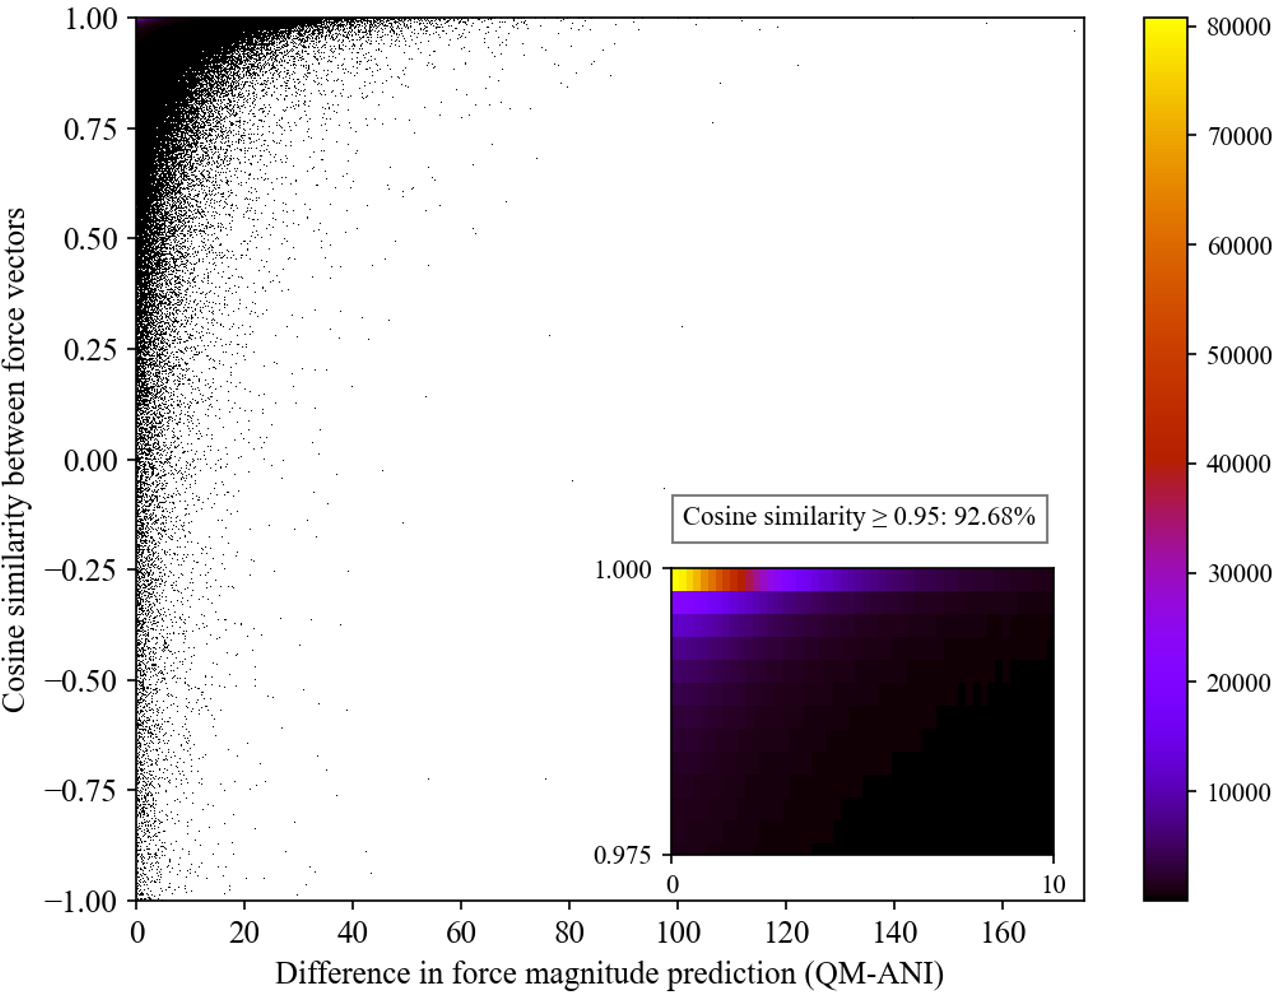
\includegraphics[width=1\linewidth]{Images/2xr_forces/cos_sim-hist2d-insert.png}
    \caption[2D histogram of cosine similarity measure of predicted atomic force vectors]{ \authorRemark{Give these different captions} \\
    Cosine similarity between ANI predicted forces (per-model) versus the DFT reference forces on the COMP6v1 benchmark dataset.
    }
    \label{fig:2d_2xr_comp6v1-forces-cos_sim}
\end{figure}

This metric captures the directional agreement between predicted and true force vectors, illustrating that ANI models, in nearly all cases, predict forces that align closely with the correct direction on the PES. 
Even in cases where predictions deviate, these errors tend to occur in low-error structures near equilibrium, where the magnitude of the force vector is very small. 
This suggests that while absolute force magnitudes vary across the ensemble, the network reliably captures the qualitative features of the PES.
The cosine similarity data is re-plotted in three dimensions in Figure \ref{fig:2xr_comp6v1-forces-cos_sim}, further demonstrating the directional agreement of predicted atomic forces.

\begin{figure}[H]
    \centering
    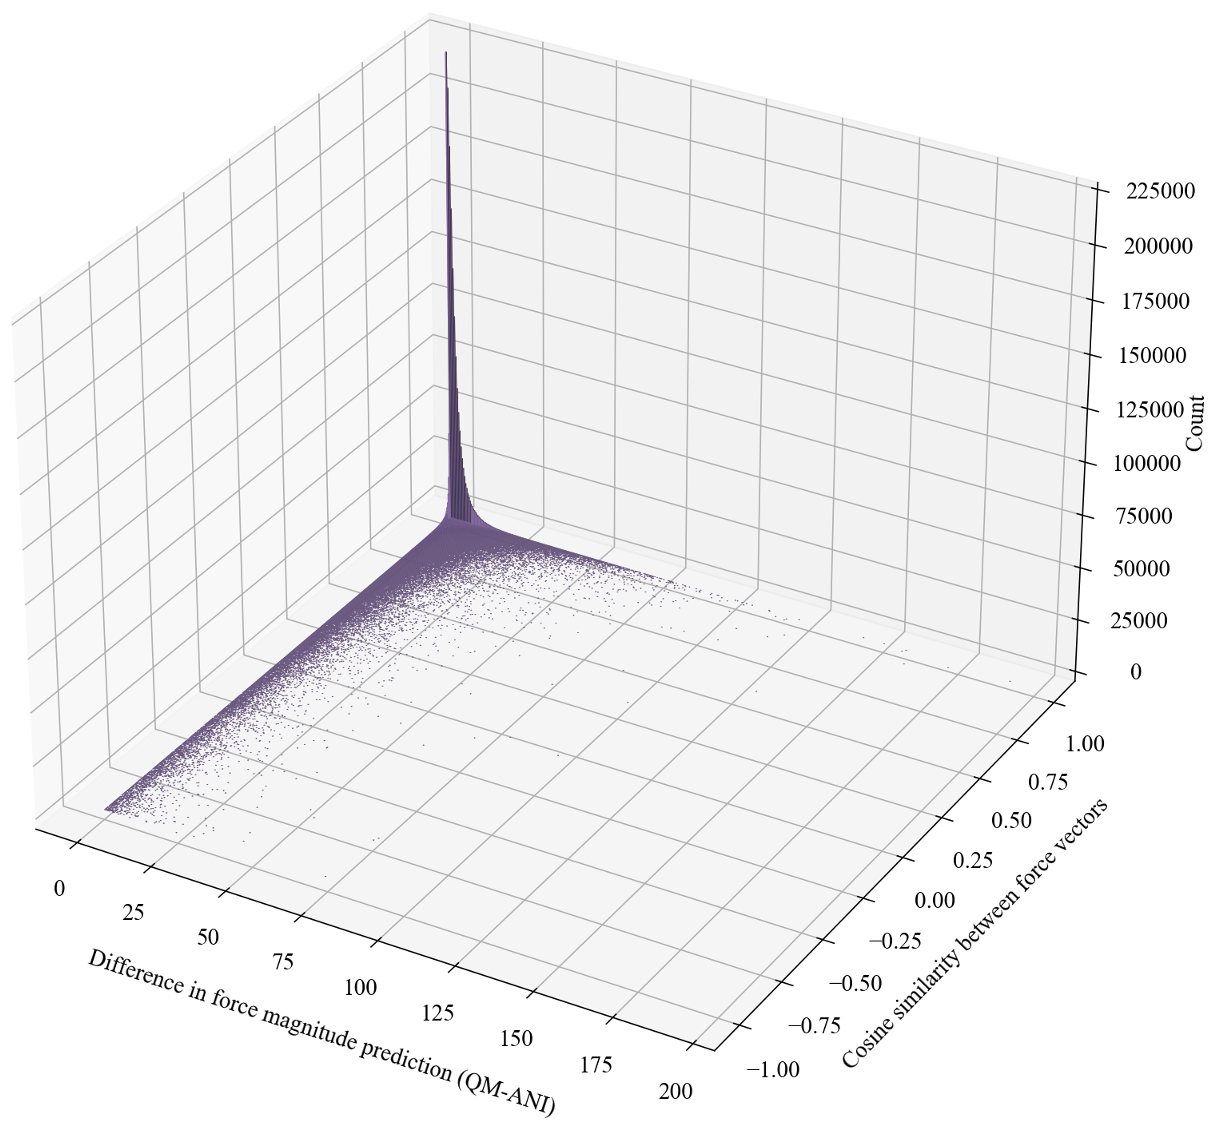
\includegraphics[width=1\linewidth]{Images/2xr_forces/2xr_comp6v1_force-cosine_sim-bar3d.png}
    \caption[3D histogram of cosine similarity measure of predicted atomic force vectors]{
    Cosine similarity between ANI predicted forces (per-model) versus the DFT reference forces on the COMP6v1 benchmark dataset.
    }
    \label{fig:2xr_comp6v1-forces-cos_sim}
\end{figure}

One of the key advantages of using force predictions for uncertainty quantification is their sensitivity to local errors in the PES. 
Atomic forces provide spatially resolved information that reflects the stability of individual atoms within their local chemical environment. 
This enables a more granular assessment of uncertainty, where high-uncertainty atoms may indicate regions of the molecule that are poorly represented in the training data. 
Additionally, because forces influence molecular motion in dynamics, uncertainty in force predictions may translate directly to instabilities in simulations, making it important to assess their reliability in MD applications.

Another consideration is the role of ensemble-based predictions in force uncertainty estimation. In ANI, force vectors are obtained independently from each model within the ensemble, meaning that variations in force predictions across the ensemble provide a direct measure of model disagreement. This disagreement can be leveraged as an uncertainty metric, where a high standard deviation in force predictions signals regions of chemical space where the model lacks confidence. Importantly, unlike atomic energies, which exhibit compensatory behavior across the ensemble (as discussed in Section \ref{sec:uncertainty_atomic_energies}), force predictions do not sum to a fixed total value. This means that force uncertainty is not artificially constrained, making it a more reliable measure of true model uncertainty rather than an artifact of network training.

Beyond uncertainty quantification, force predictions also offer practical advantages for improving the robustness of ANI models. Since forces define the shape and curvature of the PES, incorporating force-based uncertainty into active learning strategies could enhance the selection of training data, ensuring that new data points are sampled in regions of highest uncertainty. This approach has been explored in other uncertainty-aware machine learning models \cite{uncertainty_atomistic_ml_peterson}, but its application to force-driven active learning in ANI remains an open area of research.

In summary, atomic forces provide a compelling alternative to atomic energy-based uncertainty measures, offering physically meaningful, localized, and dynamically relevant information about model reliability. The strong directional agreement between ANI-predicted and reference forces demonstrates that, even in cases of mild uncertainty, the model remains faithful to the underlying physics of molecular interactions. The following sections will further explore the statistical properties of force predictions and investigate how ensemble variance can be used as a practical uncertainty metric in molecular simulations.

While atomic forces present a promising avenue for uncertainty quantification, they also introduce a new challenge: each atom's force prediction consists of three independent vector components, corresponding to the 
$x$,$y$, $z$ directions. Unlike total energy, which is a scalar quantity that can be directly compared across different molecules, force vectors introduce dimensional complexity when attempting to reduce uncertainty to a single measure. A meaningful uncertainty metric must distill this multi-component information into a single scalar value that captures the reliability of force predictions without discarding essential physical details.

Force vectors inherently contain two distinct aspects: direction and magnitude. In the previous analysis, we evaluated force directionality by considering cosine similarity between predicted and reference force vectors. This measure allowed us to assess how well the ANI models capture the qualitative structure of the potential energy surface, ensuring that forces point in the correct directions even when individual model predictions differ. However, directional agreement alone does not provide a complete picture of uncertainty—forces with similar orientations may still differ significantly in magnitude.

To develop a comprehensive force-based uncertainty measure, it is necessary to investigate the second aspect of force predictions: magnitude variations across the ensemble. If models in the ensemble consistently predict similar force magnitudes, we can infer that the model is making confident predictions in that region of chemical space. Conversely, if the ensemble exhibits high variance in force magnitudes, this suggests increased uncertainty, potentially indicating that the model has encountered an unfamiliar molecular environment.

The following sections will focus on force magnitude variability as a key metric for uncertainty estimation. By examining how force magnitudes fluctuate across the ensemble, we aim to construct a single, physically meaningful uncertainty measure that accounts for both the direction and strength of predicted atomic interactions.

\subsection{Force Magnitudes}
\label{subsec:force_magnitudes}

While the previous section demonstrated that ANI models accurately predict the direction of atomic forces, an equally important aspect of force reliability is their magnitude. The magnitude of an atomic force vector determines how strongly an atom is being pulled or pushed within the potential energy surface (PES), making it a crucial factor in molecular dynamics simulations, vibrational analysis, and transition state searches. If a neural network potential (NNP) systematically underestimates or overestimates force magnitudes, it could lead to errors in predicted reaction kinetics, structural stability, or even failures in long-time dynamical simulations.

\begin{figure}[H]
    \centering
    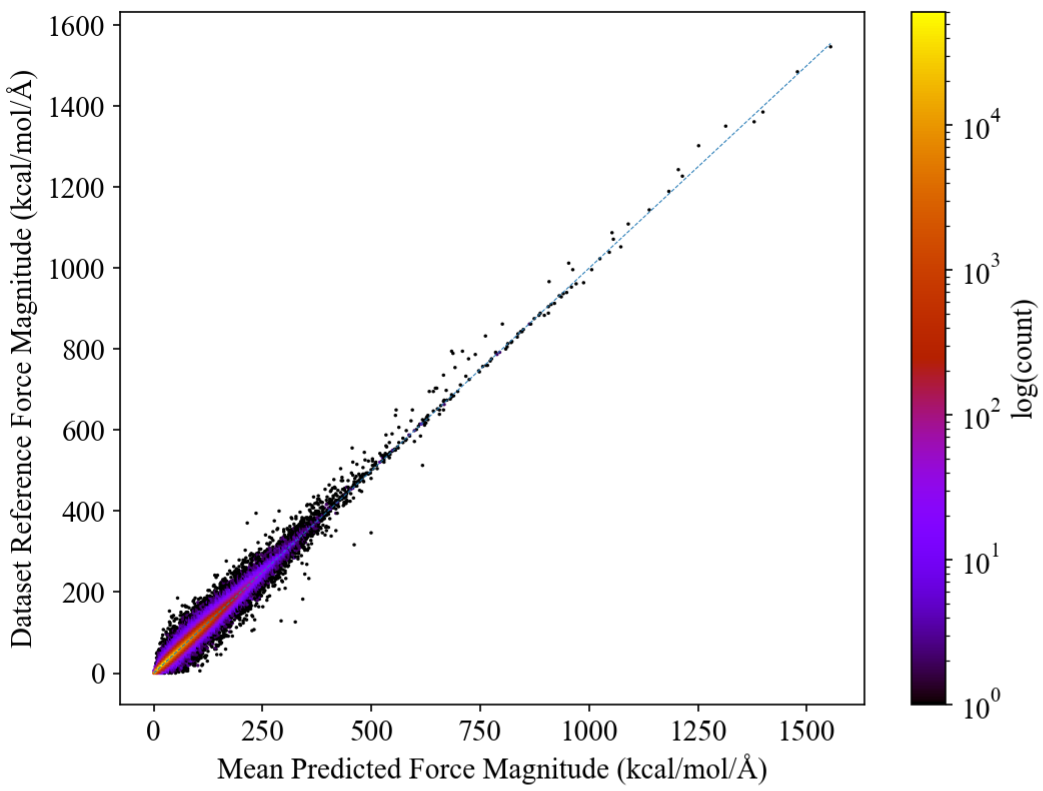
\includegraphics[width=1\linewidth]{Images/2xr_forces/2xr_comp6v1_force-dft-vs-mean_ani.png}
    \caption[Mean predicted atomic force magnitude vs DFT reference]{Predicted force magnitudes vs DFT reference force magnitudes on the COMP6v1 benchmark dataset.}
    \label{fig:2xr_comp6v1-forces-ani_vs_ref}
\end{figure}

Figure \ref{fig:2xr_comp6v1-forces-ani_vs_ref} presents a comparison between the mean force magnitudes predicted by ANI-2x models and the corresponding reference DFT forces. The near-perfect correlation indicates that ANI is not only capable of capturing the qualitative structure of the PES but also reproduces the quantitative force magnitudes with remarkable accuracy. This suggests that ANI models, despite being trained primarily on total energy loss functions, inherently learn force relationships with high precision. The success of ANI in predicting force magnitudes reinforces its applicability for molecular simulations where atomic forces dictate physical behavior, ensuring that molecular geometries evolve realistically under machine-learned potentials.

Given this high level of accuracy, one might initially question whether force magnitudes could serve as an effective uncertainty measure. After all, if ANI reliably reproduces DFT-level force magnitudes, does this not indicate that its uncertainty is already minimized? However, a strong mean prediction does not necessarily preclude fluctuations at an individual atomic or molecular level, particularly across different models in the ensemble. The figure only represents the mean force magnitudes over all molecules in the dataset, without accounting for per-atom variability or systematic differences among individual models. Therefore, while ANI performs well on average, ensemble disagreement may still highlight regions of higher uncertainty, even in cases where the mean force magnitude closely aligns with the DFT reference.

One potential avenue for force-based uncertainty quantification is to examine the variance in predicted force magnitudes across the ensemble. Since the ANI methodology employs multiple independently trained neural networks, predictions for a given molecule are not derived from a single deterministic function but rather from an ensemble of models, each trained on slightly different data distributions and weight initializations. This introduces a natural measure of model uncertainty: when all models predict similar force magnitudes, the uncertainty is low, but when the predicted forces fluctuate across the ensemble, it signals that the model is less confident in that region of chemical space. This principle has been widely explored in the uncertainty literature \cite{uncertainty_atomistic_ml_peterson, uncertainty_of_nnp_ensembles_kahle}, but its specific application to force magnitudes in ANI models remains underdeveloped.

A second approach to leveraging force magnitudes for uncertainty estimation involves examining force magnitude outliers in chemically or structurally unusual environments. In equilibrium geometries, where atomic forces are inherently small, the variance in predicted forces may be less informative. However, in transition states, strained geometries, or reactive molecular conformations, force magnitudes often become large due to steep gradients in the PES. If ANI exhibits greater uncertainty in force magnitudes for these structures—particularly in cases where training data is sparse—this could indicate a fundamental limitation of the model in extrapolating beyond its training regime. Investigating this phenomenon could reveal whether large force magnitude uncertainty correlates with high prediction error in chemically meaningful ways.

Furthermore, force magnitudes provide a local, per-atom uncertainty measure that is inherently more granular than molecular energy-based uncertainty metrics. Unlike total energy, which represents a global property of a molecule, atomic forces vary from one atom to another within the same structure. This means that force-based uncertainty estimates could highlight specific atomic sites where the model is less confident, rather than giving a single uncertainty value for an entire molecule. This property makes force magnitudes an appealing candidate for identifying underrepresented chemical environments in a dataset, as regions with large force magnitude variance could indicate where additional data collection or active learning efforts should be focused.

Ultimately, while Figure \ref{fig:2xr_comp6v1-forces-ani_vs_ref} demonstrates that ANI’s force predictions are highly accurate, this analysis alone does not reveal the full picture of force-based uncertainty. The next step is to explore atomistic measures of uncertainty derived from force magnitudes, specifically by evaluating how force predictions fluctuate across models in the ensemble and whether these fluctuations serve as reliable indicators of model confidence. The following sections will focus on quantifying force-based uncertainty, assessing whether per-atom force variance correlates with true model error, and determining whether this approach offers a meaningful improvement over traditional energy-based uncertainty metrics.

\section{Analyzing the Uncertainty of Force Predictions}
\label{sec:analyzing_force_uncertainty}

Quantifying uncertainty in force magnitude predictions presents a significant challenge due to the wide variability of force magnitudes across different atomic environments. Since force magnitudes naturally depend on both atom type and the extent to which a structure deviates from equilibrium, direct comparisons across molecules or atomic species can be misleading. Ideally, a useful uncertainty measure would highlight high-energy error structures—cases where ANI predictions are unreliable—without being confounded by unrelated factors such as intrinsic force magnitude variation.

As an initial approach, we examined the standard deviation of force magnitudes across the ANI ensemble (figure forthcoming). While this metric does capture ensemble disagreement, it remains heavily biased by the absolute size of the force vectors—atoms experiencing large forces tend to have larger standard deviations, even when the model’s predictive confidence is high. To account for this, we next considered the coefficient of variation (relative standard deviation) in Equation \ref{eq:rel_stdev} defined as the standard deviation of force magnitudes divided by the mean force magnitude:

\begin{equation} 
\text{Relative standard deviation} = \frac{\sigma_{|\vec{F}|}}{\mu_{|\vec{F}|}}
\label{eq:rel_stdev}
\end{equation}

This normalization helps to mitigate the absolute magnitude dependence, but still shows strong correlations with vector size, as evidenced in Figure \ref{fig:2xr_comp6v1-force_uncertainty-violin}. Large force magnitudes, even when well-predicted, tend to exhibit higher relative standard deviations, limiting the ability of this metric to consistently identify high-error regions.

To further refine the approach, we introduced an alternative measure: the relative range (Eqn. \ref{eq:rel_range}), which captures the spread of predicted force magnitudes across the ensemble, relative to the mean force magnitude:
\begin{equation} 
\text{Relative range} = 
\frac{\max \left( |\vec{F}| \right) - \min \left( |\vec{F}| \right)}
                            {\mu_{|\vec{F}|}} 
\label{eq:rel_range}
\end{equation}

This metric (right panel of Figure \ref{fig:2xr_comp6v1-force_uncertainty-violin}) effectively scales the spread of force predictions to the mean, reducing the bias toward large-magnitude forces while still reflecting ensemble disagreement. Compared to relative standard deviation, relative range appears less dependent on force magnitude size, making it a potentially more reliable uncertainty quantifier.
However, to determine whether these force-based uncertainty measures provide meaningful insight into ANI model confidence, we must assess their relationship with total molecular energy error. 

\begin{figure}[H]
    \centering
    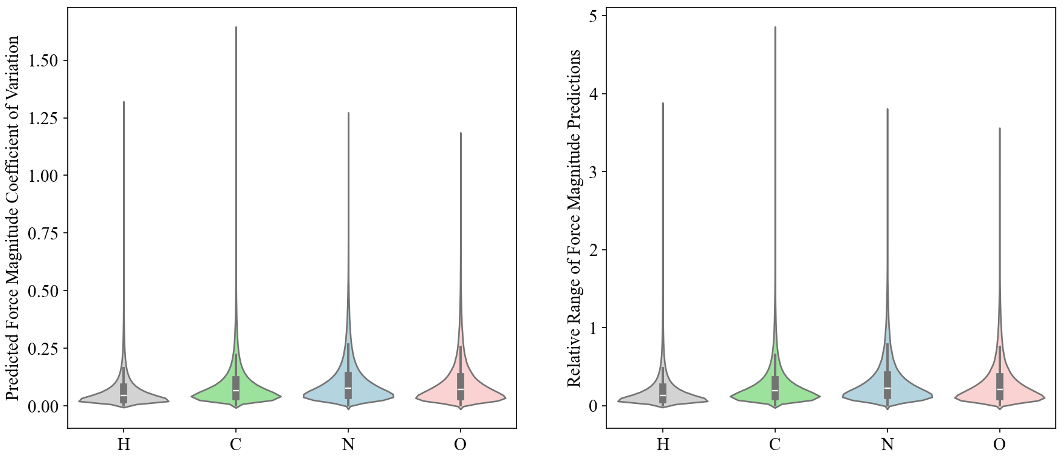
\includegraphics[width=1\linewidth]{Images/2xr_forces/2xr_comp6v1_force-uncertainty_violin.png}
    \caption[Uncertainty in force magnitude predictions: violin distribution]{Violin distribution of force magnitude uncertainty measures (relative standard deviation and relative range), computed for ANI-2xr predictions on the COMP6v1 benchmark dataset.}
    \label{fig:2xr_comp6v1-force_uncertainty-violin}
\end{figure}

Figure \ref{fig:2xr_comp6v1-mean_force_uncertainty_hexbin} presents a direct comparison between per-molecule averaged force uncertainty measures and energy error on the COMP6v1 benchmark dataset. If a clear correlation emerges, these metrics could serve as practical, physics-based uncertainty estimators, enabling more reliable assessments of ANI model reliability without requiring external validation data.

\begin{figure}[!hp]
    \centering
    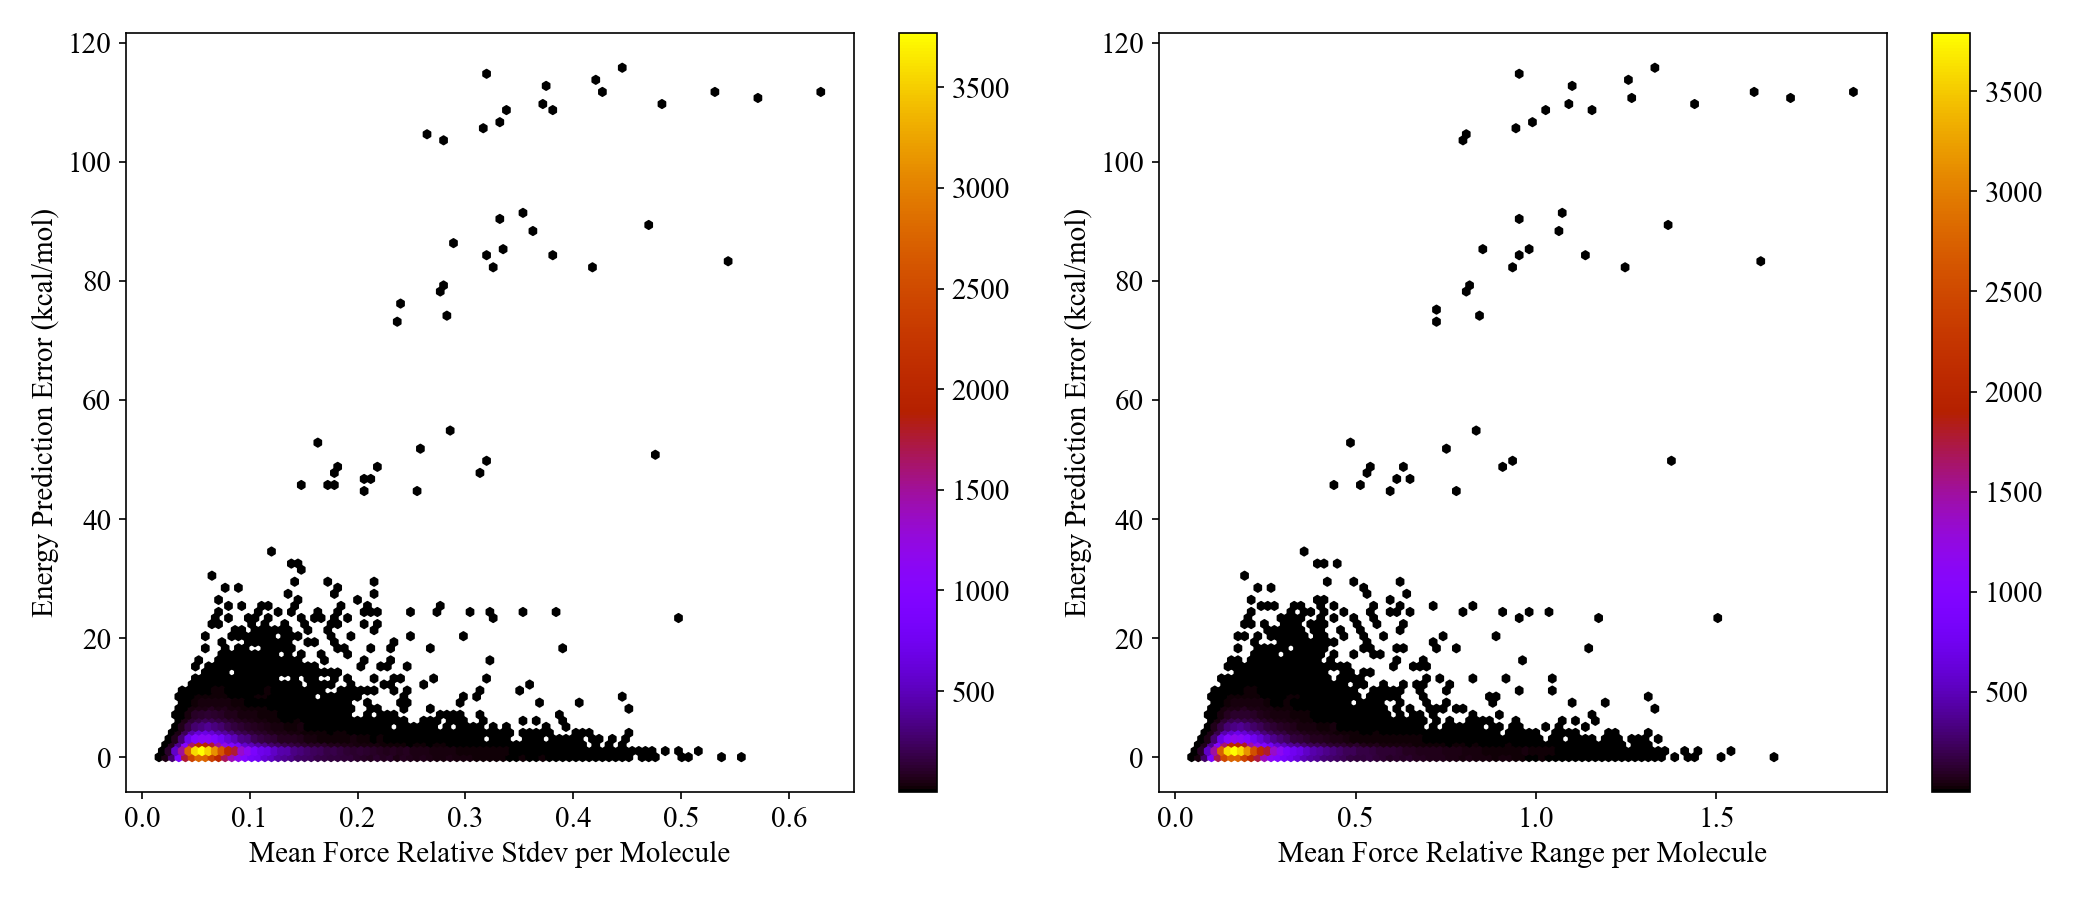
\includegraphics[width=1\linewidth]{Images/2xr_forces/2xr_comp6v1_force-mean-uncertainty-vs-energy.png}
    \caption[Average force uncertainty measures per-molecule versus energy error (COMP6v1)]{Averaged uncertainty measures per-molecule on the ANI-2xr predicted forces versus the energy error for the COMP6v1 benchmark dataset.}
    \label{fig:2xr_comp6v1-mean_force_uncertainty_hexbin}
\end{figure}

To refine our approach further, we explored alternative methods of aggregating atomic force uncertainties at the molecular level. One possibility was to assign greater importance to highly uncertain atomic forces when computing per-molecule uncertainty scores. Figure \ref{fig:2xr_comp6v1-mean_force_uncertainty_hexbin} presents the results of a straightforward averaging approach, where each molecule's force uncertainty is computed as the mean of its atomic uncertainties. While this yielded a reasonable correlation with molecular energy error, we hypothesized that higher-uncertainty atomic forces might contribute disproportionately to poor energy predictions.

To test this, we introduced exponential weighting of atomic force uncertainty measures, increasing the influence of large deviations when computing molecular-level uncertainty. The weighted mean was computed using an exponential function is given in Eqn. \ref{eq:outliers-weighted_sum}.

\begin{equation} 
\mu_{\text{weighted}} = \frac{\sum_i u_i e^{\alpha w_i}}{\sum_i e^{\alpha w_i}} 
\label{eq:outliers-weighted_sum}
\end{equation}

Where $\mu_i$ represents an atomic uncertainty measure (relative standard deviation or relative range), and $w_i$ is a weighting factor, with an adjustable hyperparameter $\alpha$ controlling the strength of weighting. The goal was to emphasize large deviations in atomic force predictions, ensuring that molecules with a few highly uncertain atomic forces would be flagged as high-error cases.


\begin{figure}[!hp]
    \centering
    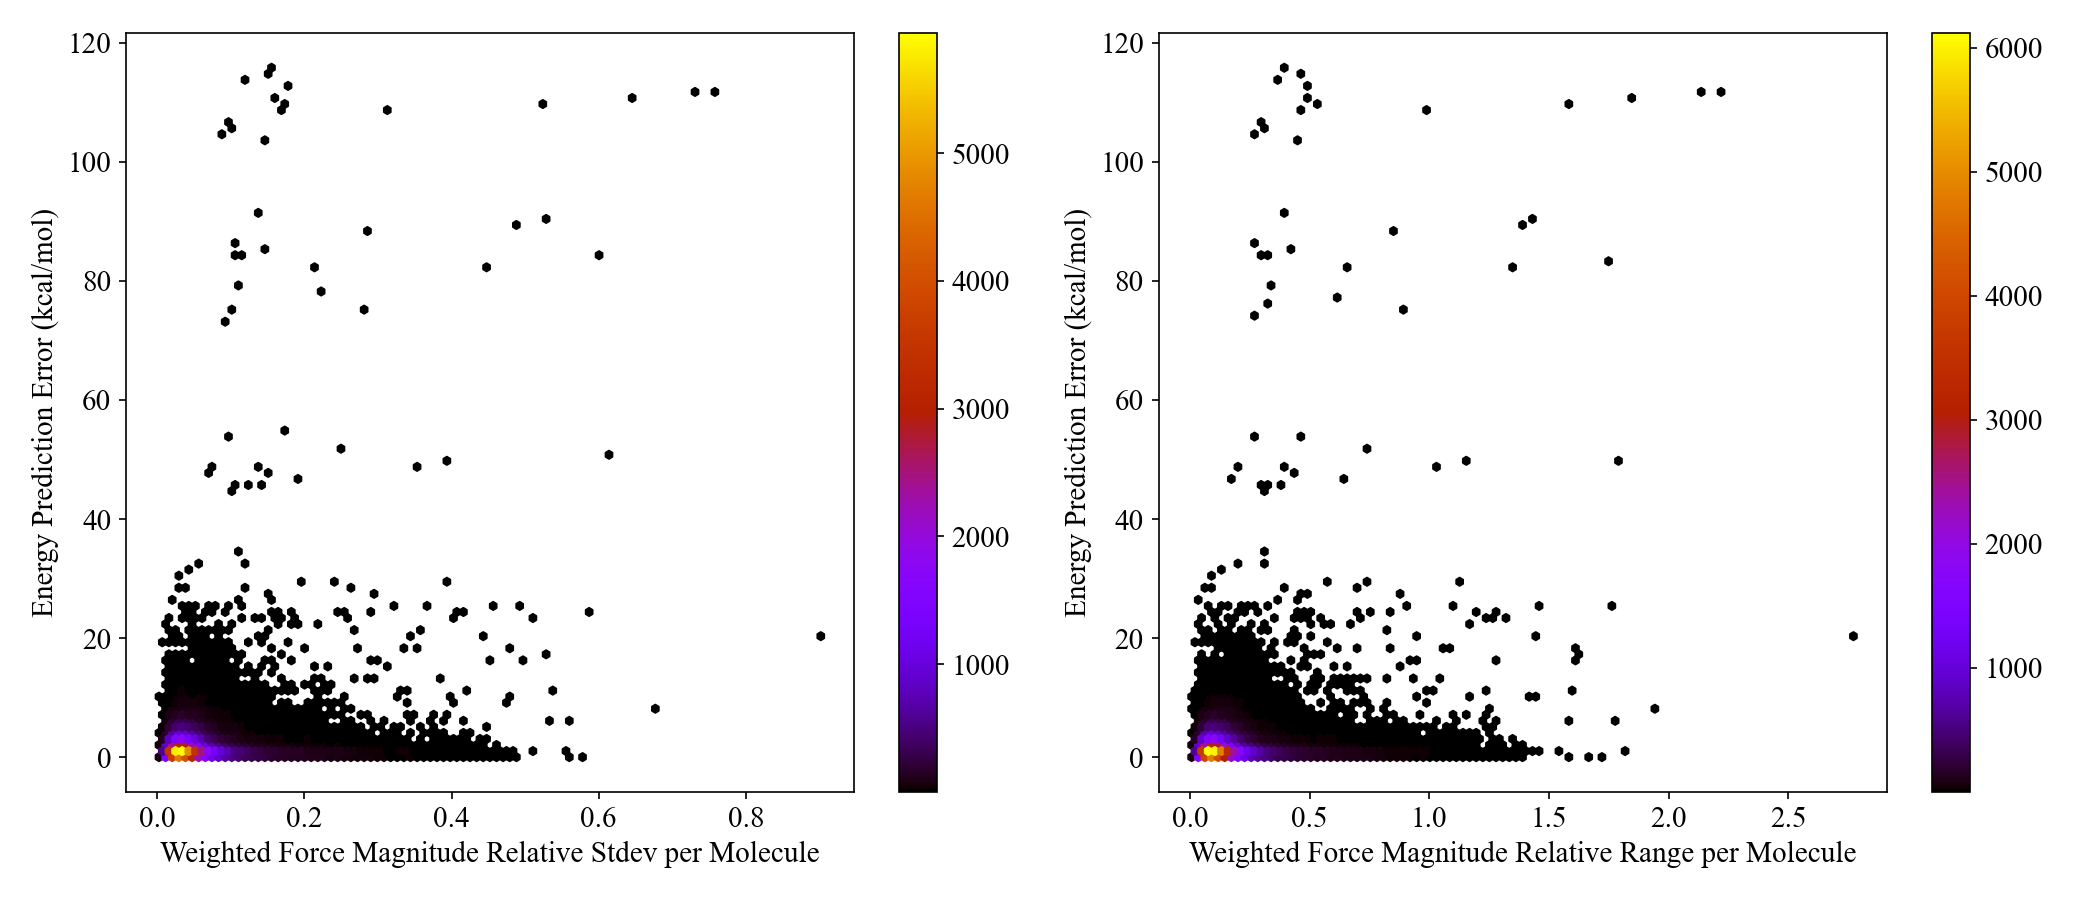
\includegraphics[width=1\linewidth]{Images/2xr_forces/2xr_comp6v1_force-weighted-uncertainty-vs-energy.png}
    \caption[Force uncertainty weighted by outliers versus energy error (COMP6v1)]{Outlier-weighted uncertainty measures for ANI-2xr predicted force magnitudes versus the energy error on the COMP6v1 benchmark dataset.}
    \label{fig:2xr_comp6v1-forces-weighed_uncertainty}
\end{figure}

However, Figure \ref{fig:2xr_comp6v1-forces-weighed_uncertainty} shows that this approach performed worse than simply averaging per-atom uncertainties. The exponential weighting appeared to overemphasize localized outliers, reducing the correlation with molecular energy error rather than improving it. This suggests that large atomic force deviations alone are not always indicative of high molecular uncertainty, and that a different approach was needed.

Given the shortcomings of our weighting approach, we instead focused on capturing the largest single force deviation per molecule. The maximum deviation metric is defined in Equation \ref{eq:max_force_deviation}.

\begin{equation} 
\text{Max deviation} = 
\frac{\left| \left(\max\limits_{m \in {1, \dots, 8}} \vec{F}_{\text{ANI}}^m \right)- \mu_{\text{ANI}} \right|}{\mu_{\text{ANI}}} 
\label{eq:max_force_deviation}
\end{equation}

Where $\vec{F}_{\text{ANI}}^m$ represents the predicted force vector from the $m^{\text{th}}$ model in the ANI ensemble and $\mu_{\text{ANI}}$ represents the mean predicted force magnitude for a given atom across the 8-model ensemble, ensuring that deviations are evaluated relative to the overall prediction spread. The maximum deviation captures the single most extreme disagreement among the ensemble members, highlighting cases where one model significantly diverges from the consensus. By normalizing this deviation by the mean force magnitude, this metric prevents small-force predictions (e.g., near equilibrium) from being overshadowed by inherently larger forces, making it a scale-invariant measure of uncertainty.

Figure \ref{fig:2xr_comp6v1-forces-highest_deviation} presents this maximum deviation measure against molecular energy error. Unlike earlier approaches, this metric highlights cases where at least one atomic force prediction deviates significantly from the ensemble consensus, offering a strong correlation with molecular energy uncertainty.

\begin{figure}[!ht]
    \centering
    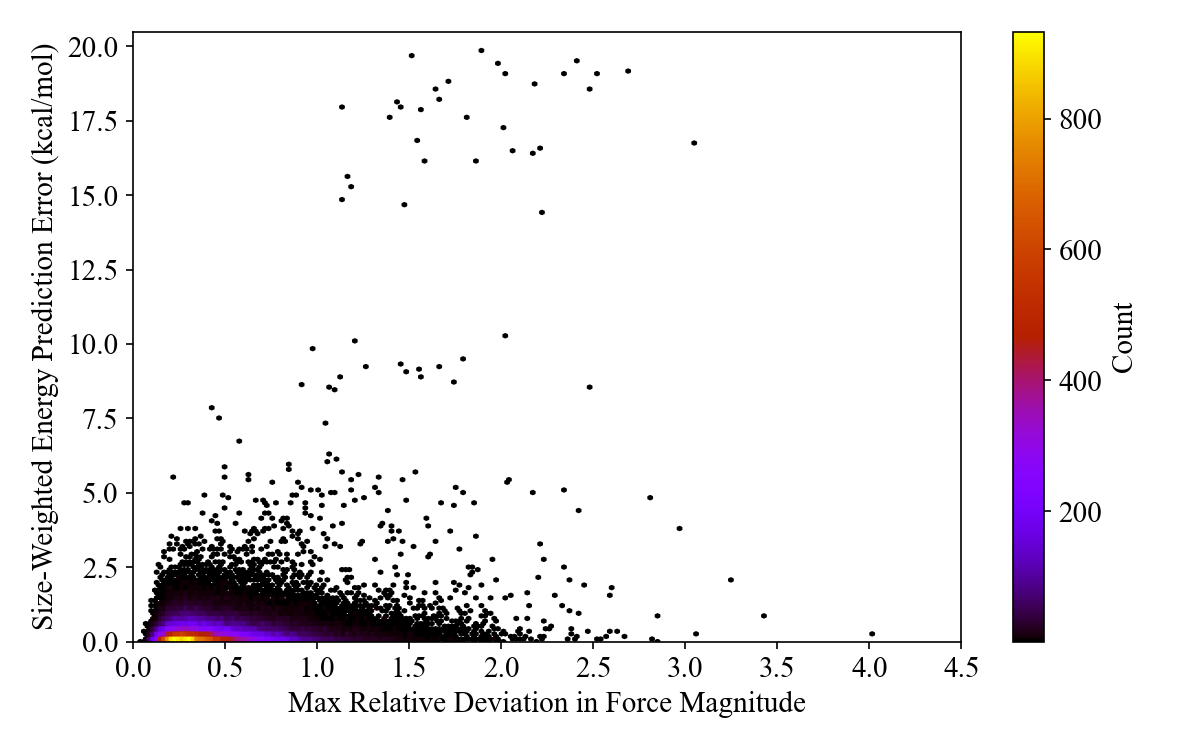
\includegraphics[width=1\linewidth]{Images/2xr_forces/2xr_comp6v1_force-highest-force_deviation-vs-energy.png}
    \caption[Maximum deviation in force magnitude prediction versus energy error (COMP6v1)]{Maximum deviation in force magnitude prediction by ANI-2xr versus energy error on the COMP6v1 benchmark dataset.}
    \label{fig:2xr_comp6v1-forces-highest_deviation}
\end{figure}

The results in Figure \ref{fig:2xr_comp6v1-forces-highest_deviation} demonstrate that the maximum deviation in force magnitude prediction serves as a robust indicator of molecular energy uncertainty. Unlike earlier uncertainty measures that were biased by intrinsic variations in force magnitude, this metric specifically identifies cases where at least one atomic force prediction deviates significantly from the ensemble mean, highlighting regions of the molecule where the model exhibits low confidence. This suggests a crucial improvement to the active learning framework: rather than selecting new training data based on the total energy uncertainty of an entire molecular conformation, we can refine the Query by Committee (QBC) process to target high-uncertainty atomic regions.

The original ANI-1x active learning strategy \cite{ani-1x} leveraged energy-based QBC to identify and sample high-uncertainty molecular structures. However, this approach is limited by its molecule-wide uncertainty aggregation, meaning it treats an entire molecule as either well-represented or underrepresented in the training data. Our findings suggest a more efficient sampling strategy: instead of selecting entire molecules based on total energy uncertainty, we can prioritize the specific conformations where atomic forces exhibit high model disagreement. By refining the active learning process to focus on atomic force uncertainty, we could accomplish three things. (1) Reduce the total amount of required training data while maintaining ANI’s predictive accuracy, similar to the "less is more" approach demonstrated in ANI-1x. (2) Ensure that newly sampled molecules contribute maximally to improving model generalization, by filling in high-uncertainty regions of atomic interactions rather than redundantly adding molecules that contribute little new information. (3) Improve transferability to unseen chemical systems by strategically selecting only the conformers that challenge the model, enhancing its ability to generalize beyond its training set.

The overarching goal is to make ANI equally powerful with less data—a principle demonstrated by the effectiveness of the ANI-1x dataset, which achieved lower molecular energy prediction errors using only a fraction of the original ANI-1 dataset. Applying a similar data-efficient philosophy to force-based uncertainty could significantly accelerate ANI model training and expand its applicability to larger and more diverse chemical spaces. Future iterations of ANI training could incorporate force-based uncertainty quantification into the active learning pipeline, refining data selection to directly address the weakest points of the model. This would not only reduce computational costs but also enhance the overall accuracy and reliability of ANI predictions, ensuring more consistent performance across a wider range of molecular systems.

Having established that atomic force uncertainty serves as a reliable indicator of molecular energy error, the next logical step is to develop a framework for systematically isolating and refining these high-uncertainty regions. Instead of selecting entire molecular structures for retraining, we propose a method to extract and focus on the specific atomic environments that contribute most to uncertainty—a process that could drastically improve the efficiency of the active learning pipeline.

\subsection{Atom Isolator}
\label{subsec:atom_isolator}

To this end, we began developing a tool called Atom Isolator, designed to automatically identify and extract high-uncertainty atoms from molecular structures. The goal of this approach is to refine the active learning process by targeting specific atomic environments rather than entire molecular conformations, thereby improving model accuracy with a smaller, more informative dataset. The first step in this process is identifying high-uncertainty atoms. Using the maximum deviation in force magnitude prediction as a metric, we flag atoms where ensemble disagreement exceeds a given threshold, indicating unreliable model predictions. 

These flagged atoms represent regions where the model is least confident in its force predictions and are therefore the most critical areas to improve. Once these high-uncertainty atoms are identified, the next challenge is truncating the molecular environment in a way that preserves relevant chemical context. Extracting only the flagged atoms would result in a loss of structural information necessary for meaningful predictions. To prevent this, Atom Isolator defines a tunable cutoff radius around each high-uncertainty atom, set to approximately 1.5 times the AEV cutoff. 
An example of this is given in Figure \ref{fig:atom_isolator}.

\begin{flushleft}
\begin{multiFigure}
\begin{centering}
    \addFigure{0.4}{Images/atom_isolator/c2h3n7o2-cropped.png}
    \addFigure{0.4}{Images/atom_isolator/c2h3n7o2_highlighted-cropped.png} 
    \addFigure{0.4}{Images/atom_isolator/c2h3n7o2_11isolator-cropped.png}
    \addFigure{0.4}{Images/atom_isolator/c2h3n7o2_2isolator-cropped.png} \\
\captionof{figure}[Example output from the atom isolator]{(A) C\textsubscript{2}H\textsubscript{3}N\textsubscript{7}O\textsubscript{2} molecule from ANI dataset, (B) atoms with a high force uncertainty value, and the atom isolator output from (C) atom 2 and (D) atom 11. Note that some of the molecule is truncated at the AEV cutoff in either case; refer to Fig. \ref{fig:aev_radius} for an example of this cutoff radius.
}
\label{fig:atom_isolator}
\end{centering}
\end{multiFigure}
\end{flushleft}

\authorRemark{This ensures that enough of the local atomic environment is retained to maintain chemically meaningful interactions, while avoiding unnecessary contributions from well-learned regions of the molecule. Finally, these extracted atomic environments are treated as independent molecular fragments, which can be reintroduced into the training process. By isolating and refining only the most uncertain atomic regions, this approach prioritizes data sampling where the model struggles most, rather than redundantly retraining on entire molecular structures that contain many well-predicted regions. This focused data augmentation strategy has the potential to significantly reduce dataset size while maintaining or even improving predictive accuracy.}


The process of isolating high-uncertainty atomic environments presents an opportunity to search for reduced molecular representations that retain the key chemical patterns associated with high-uncertainty predictions. Instead of retraining the ANI model on large, computationally expensive structures, we can use these fragmented environments to identify simpler molecular motifs that capture the essential bonding interactions contributing to uncertainty. This approach aligns with broader trends in molecular AI research, where efforts to develop compressed molecular representations have led to advances in AI-driven drug discovery \cite{mol_reps_in_AI_drug_discovery_david} and systematic chemical pattern matching through SMILES and SMARTS representations \cite{SMILES_pair_encoding_li, mol_patterns_SMARTS_schmidt, automated_fragment_gen_smiles_bilsland}.

One potential application of this method is to build a database of high-uncertainty motifs, which could guide targeted data augmentation by focusing additional QM calculations on molecular substructures that ANI struggles to learn. By leveraging direct chemical perception techniques, such as those proposed by Mobley et al. \cite{direct_chem_perception_mobley}, we could further refine how we define chemically relevant fragments, moving away from conventional atom-typing approaches in favor of AI-driven adaptive fragmentation. An additional challenge in this workflow is ensuring that the truncated molecular fragments remain chemically valid after removal from their original structure. When an atom is extracted from a larger molecule, its local bonding environment is disrupted, potentially leading to unrealistic chemical representations. To address this, we explored capping the truncated fragments with hydrogen atoms, a common strategy in force field parametrization and molecular fragmentation \cite{protein_ff_fragmentation_nn_wang}.

Hydrogen capping provides a straightforward way to satisfy valency constraints and maintain a chemically reasonable representation of the isolated substructure. However, this modifies the local atomic environment, altering the AEV input representation that the ANI model originally learned from. This poses a fundamental challenge: while capping ensures that the fragment is a well-defined molecule, it may no longer resemble the high-uncertainty environment that necessitated its selection in the first place. To mitigate this issue, we investigated identifying neighboring atoms beyond the AEV cutoff radius and incorporating their influence into the truncated system. The idea was that, rather than directly capping with hydrogen atoms, we could preserve electronic effects from adjacent atoms by selecting neighbors beyond the standard AEV interaction range. This would maintain the fragment’s chemical context without introducing artificial changes to its bonding patterns.

Developing an automated approach to extracting and refining high-uncertainty fragments could significantly improve active learning strategies for ANI models. By focusing on substructures that contribute most to model uncertainty, we can enhance predictive accuracy while minimizing computational cost. Future work will involve integrating pattern-recognition algorithms for detecting recurring uncertainty motifs, leveraging SMILES-based matching methods \cite{SMILES_pair_encoding_li} to identify chemically similar environments that may require additional training data. Ultimately, Atom Isolator represents a step toward precision-driven model refinement, where retraining efforts are concentrated on the most challenging chemical motifs rather than entire molecules. By developing a framework that systematically isolates, refines, and reintegrates uncertain atomic environments, we aim to reduce dataset redundancy while improving the robustness and generalizability of ANI predictions.

\subsection{Drawback: Configurational Sampling}
\label{subsec:drawback_config_sampling}

While the Atom Isolator approach offers a focused strategy for identifying and retraining high-uncertainty atomic environments, it presents a fundamental limitation: the lack of diverse configurational sampling. By extracting and truncating molecular substructures, we improve the representation of high-error atomic environments but do little to expand the broader diversity of molecular configurations that ANI encounters during inference. This raises a crucial question: Is targeting only localized uncertainty enough to enhance the generalizability of ANI models, or do we also need a systematic way to introduce new molecular configurations?

A fundamental distinction in molecular datasets is the difference between conformational and configurational diversity. Conformational sampling refers to generating different 3D structures (rotamers) of a given molecule, such as exploring torsional rotations around flexible bonds, bending of molecular frameworks, or sampling vibrational distortions near equilibrium geometries. While this form of sampling is important, it is inherently limited to a fixed set of molecular graphs, meaning that it does not expand the diversity of molecular connectivity patterns available to the model. Historically, ANI datasets—including ANI-1 \cite{ani-1} and ANI-2x \cite{ani-2x}—have relied heavily on conformational sampling to enrich training data. The molecules in these datasets were sourced from large enumerated molecular databases, such as GDB-13 \cite{gdb-13} and GDB-17 \cite{gdb-17}, which contain systematic lists of all possible stable organic molecules up to a given number of heavy atoms. These datasets provide exhaustive coverage of stable molecules with up to 13 or 17 heavy atoms, respectively, ensuring that small organic structures are well-represented.

However, a major issue with this approach is dataset redundancy. The GDB databases were designed for small molecule discovery and drug-like compounds, meaning that a vast majority of the structures they contain exhibit similar functional groups and molecular motifs. The result is an oversampling of certain chemical environments, leading to a model that performs well on common molecular patterns but struggles when exposed to molecules that differ significantly from those in training. The consequence of this presents a hole in configurational diversity—the model lacks exposure to entirely new molecular architectures. If we only expand the training set through conformational sampling, we remain constrained to a narrow region of chemical space, improving accuracy within that limited domain but failing to generalize beyond it. This means that ANI models will inevitably encounter molecules during inference that fall well outside their learned chemical space, leading to poor extrapolation and unreliable predictions for novel molecules.

To truly enhance ANI’s reliability, we need to go beyond conformational sampling and introduce configurational sampling—the process of systematically expanding the molecular connectivity space that the model has access to. While conformational sampling ensures that a given molecule’s low-energy geometries are well-represented, configurational sampling ensures that a model encounters diverse bonding topologies, functional group variations, and novel molecular frameworks.

A promising source of configurational diversity is ChEMBL \cite{ChEMBL_gaulton}, a large database of bioactive molecules with experimentally validated drug-like properties. Unlike GDB-derived datasets, which primarily contain small, stable organic molecules, ChEMBL includes a broader range of chemically relevant structures, including pharmacophores and complex heterocycles commonly found in medicinal chemistry, reactive intermediates and metabolites, which provide insights into chemical reactivity, and transition-state-like geometries, which are critical for understanding reaction dynamics. By incorporating ChEMBL-derived molecules into the training process, we can expand ANI’s knowledge of chemical space, enabling it to generalize more effectively to novel compounds.

Another approach to increasing configurational diversity is the systematic generation of new molecular fragments based on high-uncertainty atomic environments. As explored in the Atom Isolator section, truncated high-uncertainty regions provide insight into molecular motifs that challenge ANI’s predictions. If we can map these motifs to larger molecular frameworks, we may be able to generate new molecules that share key bonding characteristics but provide fresh chemical contexts for model training.

This discussion leads to a critical consideration: If ANI models struggle most in specific atomic environments, should active learning strategies focus on fine-tuning the model using extracted high-error substructures, or should they instead prioritize generating novel configurations that explore previously unseen regions of chemical space? The Atom Isolator approach enhances model refinement, but it does not necessarily expand the configurational diversity of the training set.

A more balanced solution may involve a hybrid approach—using high-uncertainty atomic fragments as a guide for selecting new molecular configurations from external databases, allowing the model to learn from both localized uncertainty and broader molecular diversity. This concept is explored in greater depth in Section \ref{sec:exploring_new_mol_configs}, where we examine how configurational sampling methods can be leveraged to improve ANI’s coverage of the potential energy surface.

\section{Outlook}

The exploration of uncertainty in ANI predictions has revealed both the strengths and limitations of current ensemble-based approaches. While total molecular energy uncertainty, measured via query by committee (QBC), has been a useful heuristic for active learning, our investigation has shown that atomic force uncertainty provides a more physically meaningful alternative. By shifting the focus from total energy deviations to localized force-based uncertainty measures, we have outlined a potential pathway toward more targeted and data-efficient model training strategies.

The development of the Atom Isolator provides a first step in refining active learning strategies, allowing us to focus training on high-uncertainty regions of molecular space rather than entire conformational ensembles. However, as discussed in Section \ref{subsec:drawback_config_sampling}, this approach alone does not fully address the need for configurational diversity in ANI training. Moving forward, an integrated approach—combining uncertainty-driven atomic substructure selection with configurational expansion strategies—may offer the most efficient path toward improving model generalization.

Beyond training set refinement, the uncertainty quantification methods explored in this work could also facilitate the expansion of ANI models to include additional elements, most notably phosphorus, which would enable the accurate simulation of RNA, DNA, and other biomolecular systems. The ability to systematically detect regions of high uncertainty provides a powerful tool for identifying failure modes in ANI predictions before they impact large-scale simulations. By applying these uncertainty-driven strategies, we could prioritize high-uncertainty phosphorus-containing structures for new data generation, ensuring that ANI models gain reliable predictive power in nucleotides, phosphate-containing cofactors, and other biologically relevant molecules.

With phosphorus incorporated into the ANI framework, ANI-based potentials would become directly applicable to the study of genetic materials, unlocking high-fidelity molecular dynamics (MD) simulations of RNA folding, DNA stability, and nucleotide interactions. The ability to capture long-timescale structural rearrangements in complex biomolecules—at a fraction of the computational cost of traditional quantum mechanical approaches—would significantly enhance large-scale biochemical modeling. Moreover, these improvements could extend beyond nucleic acids, refining ANI’s applicability to organophosphates, phosphate esters, and other reactive phosphorus-containing species that play critical roles in enzymatic catalysis, prebiotic chemistry, and metabolic pathways.

By leveraging physically interpretable uncertainty metrics, we can refine data selection strategies to efficiently expand ANI's chemical scope, enhance model reliability in complex biological environments, and accelerate the development of machine-learned potentials capable of scaling to new frontiers in biomolecular and reactive chemical simulations. While achieving this will require a balance between data efficiency and chemical diversity, the methods presented in this chapter suggest a clear pathway toward constructing the next generation of ANI models with significantly broader applicability.